\chapter{Introduction}

This chapter will provide an overview of pycellerator structure and functionality. 

{\tt pycellerator} has the following components, as illustrated in figure \ref{fig:structure}. The functional relationship between these components is illustrated in figure \ref{fig:scheme}. In brief, {\tt pycellerator} first reads a model file with the \textbf{parser} and converts it to an internal database. This database is then processed by the \textbf{expander} module converts the reactions in the database to their most basic form. Control is then passed to the \textbf{interpreter}, which converts the reactions to a second database of terms of terms in differential equations, and then combines all of these terms together to form a system of differential equations out of the model. Finally, the \textbf{solver} writes the system of differential equations to a python program and then runs the program, if required to perform a numerical simulation. 

\begin{figure}[ht]
\caption{Schematic of {\tt pycellerator} structure.  Dependencies on standard python libraries (such as numpy, scypy, pyparsing, sympy, etc.) are not shown.)}\label{fig:structure}
\begin{center}
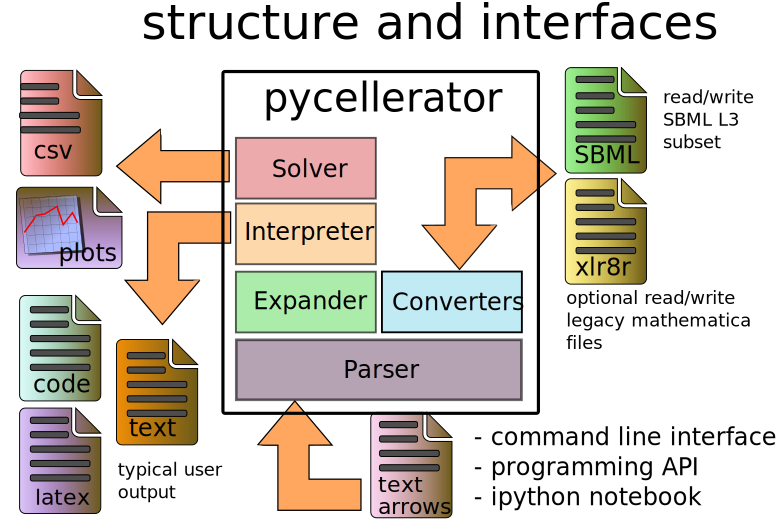
\includegraphics[width=.75\textwidth]{pyxlr8r-structure}
\end{center}
\end{figure}


\begin{description}
\item [A Parser:]

The parser module reads lists of text-formatted reactions, typically from a text file that you will manually edit by hand, that describe a particular biochemical phenomenon.  For example, a simplified version of the famous Belousov-Zhabotinsy reaction\cite{BZ1,BZ2} known as the Oregonator\cite{Oregonator1,Oregonator2} can be written in this language as:

\begin{lstlisting}
          [Br + BrO3 -> HBrO2 + HOBr, k1] 
          [Br + HBrO2 -> 2 HOBr, k2]
          [BrO3 + HBrO2 -> 2 Ce + 2 HBrO2, k3] 
          [2 HBrO2-> BrO3 + HOBr, k4] 
          [Ce -> 0.5 Br, k5]
\end{lstlisting}

The parser module converts the reactions into an internal data structure that can be interrogated by the other modules with such questions as ``What are the products of this reaction?"

The parser module is not normally invoked directly by the user. 

\item [Expander:] The expander module converts a list of complex reactions into its most basic form. For example, the input reaction

\begin{lstlisting}
	[X => Y, mod[E], rates[k1,k2,k3]]
\end{lstlisting}

is a shorthand that represents the set of biochemical reactions
\begin{align*}
\TT{X+E}&\overset{k_1}{\to}\TT{X\_E}\\
\TT{X\_E}&\overset{k_2}{\to}\TT{X+E}\\
\TT{X\_E}&\overset{k_3}{\to}\TT{X+Y}
\end{align*}
where $\TT{X\_E}$ is the name of the complex formed when {\tt E} is bound to {\tt X}.  The expander converts the input reaction to its three component reactions: 
\begin{lstlisting}
          [X+E->X_E,k1]
          [X_E->X+E,k2]
          [X_E->Y+E,k3]
\end{lstlisting}

While it is possible for the user to call the expander directly to see what the component reactions look like, usually this will be done automatically by the interpreter or solver modules and the user will generally not be required to directly interact with the expander. 

\item [Interpreter:]

The interpreter can provide a list of differential equations, a simple python program that instantiates the system of differential equations, or a \LaTeX\ representation of the system of differential equations.

The interpreter can be invoked directly, if that is what is required, but if the user is only interested in a simulation, the interpreter need not be invoked manually. 

\item [Solver:]

The primary function of the solver module is to produce a python function that is compatibly with {\tt scipy.tt.odeint}. If requested the solver module will also run a simulation utilizing the python function, plot selected (or all) simulation variables, and/or write the results to an output file in {\tt CSV} or {\tt TSV} format. Because this function is a completely stand-alone program -- fully independent of all other {\tt pycellerator} components -- multiple instantiations can be easily parallelized, e.g., for parameter optimization or other chores. 

\item [Converters:] The converters module is used to convert to and from other formats, particularly {\tt Cellerator} ({\tt xlr8r}) arrows. Every arrow implemented in {\tt pycellerator} is equivalent to some arrow in {\tt xlr8r} and vice-versa. 





\end{description}






\begin{figure}[ht]
\caption{Functional overview of {\tt pycellerator} operation. Users will interface with
{\tt pycellerator} in any of the following ways: via the {\tt pycellerator} command line interface, e.g., in the mac {\tt terminal} or or windows command prompt; in an ipython notebook; in the python shell; or by direct functions calls from other programs. 
 Every function is available via any of these techniques.  }\label{fig:scheme}
\begin{center}
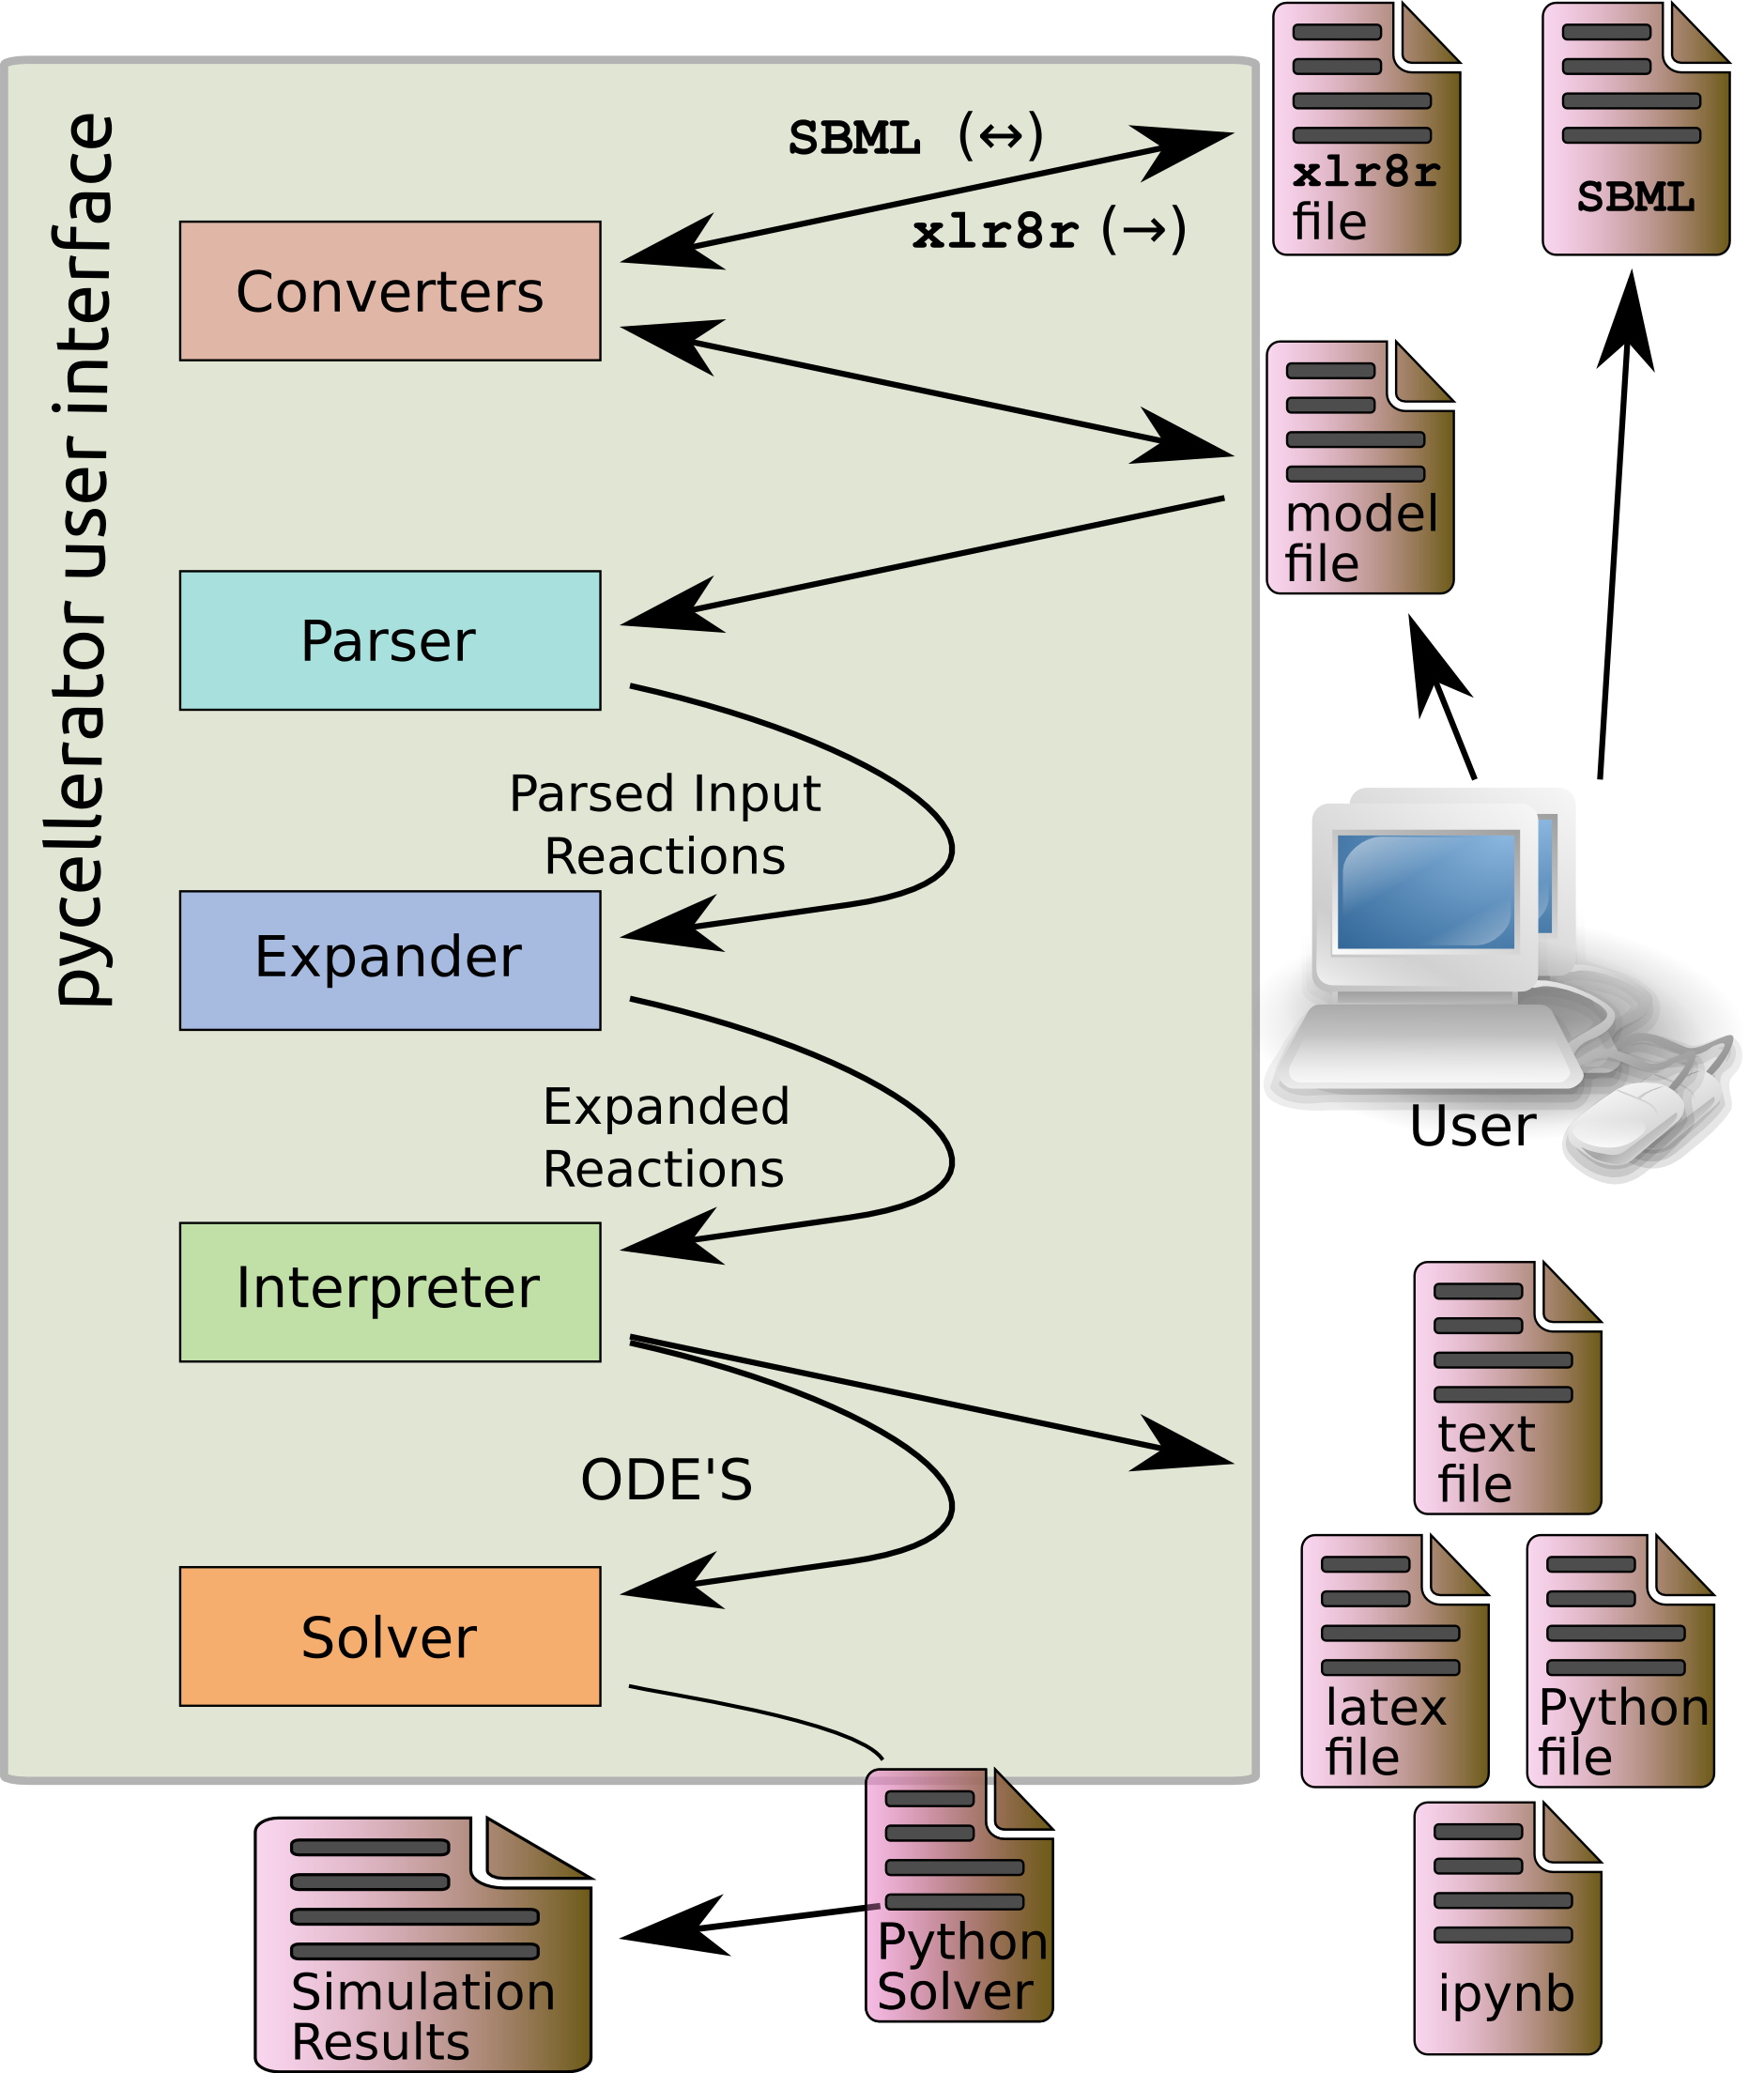
\includegraphics[width=.75\textwidth]{pyxlr8r-scheme.png}
\end{center}
\end{figure}

